
\section{Integralregning}
Nu ved vi altså, hvordan man finder hastighed og acceleration ud fra positionen, men hvis man nu kender hastigheden eller accelerationen, og man gerne vil finde positionen, hvad gør man så?
Vi har brug for det omvendte af differentialregning -- integralregning.

Integralregning er dog ikke helt så simpelt, som når man differentierer. Det skyldes, at flere \emph{forskellige} funktioner, kan have den \emph{samme} afledte. Et eksempel på dette er
\begin{equation*}
    \dv{f}{t}=\dv{}{t} \big(f(t)+k\big) \, , \, \text{hvor $k$ er en konstant} \, .
\end{equation*}
Har vi en funktion med en bestemt afledt, kan vi altid finde en ny funktion med den samme afledte ved at lægge en konstant til funktionen.

Hvis vi har en given funktion, $f(t)$, er den afledte funktion af $f(t)$, den funktion man får, når man differentierer $f(t)$.
Tilsvarende er en \emph{stamfunktion}, $F(t)$, for funktionen $f(t)$, en funktion, der har den egenskab, at dens afledte er lig med den oprindelige funktion $f(t)$.
Man finder stamfunktioner med det \emph{ubestemte integral}, som skrives
\begin{equation}
    \int f(t)\dd{t}=F(t)+k \, , \, \text{hvor} \, \dv{F}{t}=f(t).
\end{equation}
Stamfunktionerne for de fleste simple funktioner kan lures fra tabel \ref{mat:tab:diff}, og kan ses i tabel \ref{mat:tab:integral}.
\begin{table}[h]
    \centering
    \begin{tabular}{c|c|c}
    Funktionsnavn&$f(t)$&$\int f(t)\dd{t}$\\\specialrule{.125em}{.1em}{.1em}
    Konstant&$k$&$kt$\\\hline
    Potensfunktion&$t^n$&$t^{n+1}/(n+1)$\\\hline
    Reciprokfunktion&$1/t$&$\ln|t|$\\\hline
    Sinus&$\sin(t)$&$-\cos(t)$\\\hline
    Cosinus&$\cos(t)$&$\sin(t)$\\\hline
    Eksponentialfunktionen &$e^{kt}$&$e^{kt}/k$\\\hline
    Den naturlige logaritme & $\ln(t)$&$t\ln(t)-t$\\
    \specialrule{.125em}{.1em}{.1em}
    \end{tabular}
    \caption{Stamfunktioner for nogle af de mest almindelige funktioner, hvor det er undladt at lægge en tilfældig konstant til stamfunktionen. Bemærk at reglen for potensfunktioner ikke gælder, når $n=-1$.}
    \label{mat:tab:integral}
\end{table}

En af de simpleste fysiske situationer vi kan se på, er det frie fald.
Her er accelerationen konstant og lig med gravitationskonstanten
$$
a=g.
$$
Da man som tidligere nævnt finder accelerationen ved at differentiere hastigheden, må det også gælde, at hastigheden er en stamfunktion for accelerationen. Vi finder da hastigheden ud fra tabel \ref{mat:tab:integral} til at være
$$
v=\int g\dd{t}=gt+v_0 \, ,
$$
hvor $v_0$ er den tilfælde konstant for det ubestemt integral, der her angiver starthastigheden i det frie fald, altså når $t=0$. Vi finder da, at hastigheden vokser lineært med tiden.

Ligesom da vi differentierede, kan vi integrere mere komplicerede funktioner ved at tænke på dem som sammensætningere af simplere funktioner og benytte nogle regneregler for integralregning.
Integralet af en sum af funktioner er blandt andet summen af deres integraler
\begin{equation}
\int f(t)+g(t)\dd{t}=\int f(t)\dd{t}+\int g(t)\dd{t} \, .
\end{equation}
Tilsvarende kan vi sætte konstanter udenfor integraler
\begin{equation} \label{mat:eq:konstant}
\int kf(t)\dd{t}=k\int f(t)\dd{t} \, .
\end{equation}
Med disse basale integrationsregler\footnote{Det er også muligt at håndtere produktet af funktioner (delvis integration) og funktioner af funktioner (integration ved substitution), men det er mere kompliceret en for differentiering.} kan vi også finde positionen i vores eksempel
$$
x=\int v\dd{t}=\int gt+v_0\dd{t}=\frac{1}{2}gt^2+v_0t+x_0 \, ,
$$
hvor $x_0$ her er state positionen til tiden $t=0$.

\subsection{Integraler og arealet under en graf}

Ligesom differentialkvotienter (afledte) giver hældningen af grafen for en funktion, er der også en grafisk fortolkning af integraler.
Lad os sige at vi har en funktion $A(x)$, der giver os arealet under en graf $f(x)$ (målt fra $x=0$), og lad os prøve at finde denne funktions afledte.
\begin{figure}[h]
    \centering
    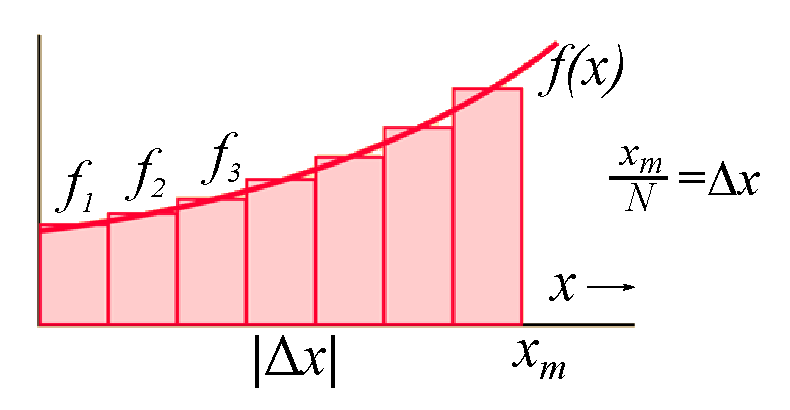
\includegraphics[width = 0.7\textwidth]{Mat/matfig/integral.eps}
    \caption{Arealet under grafen $f(x)$ tilnærmet ved at dele det op i rektangler. Kilde: \cite{Integral}.}
    \label{mat:fig:integralapprox}
\end{figure}

Hvis vi nu kigger på arealet under grafen for $f(x)$ i et interval $[x,x+\Delta x]$ på $x$-aksen, vil det være givet ved $A(x+\Delta x) - A(x)$. Dette areal må også være næsten den samme som arealet af en firkant med højden $f(x)$ og bredten $\Delta x$, se figur \ref{mat:fig:integralapprox}. Vi har da at 
$$
A(x+\Delta x) - A(x) \approx f(x)\Delta x \qquad \Rightarrow \qquad \frac{A(x+\Delta x) - A(x)}{\Delta x} \approx f(x) \, ,
$$
hvor $\approx$ betyder, at siderne er næsten lig med hinanden. Jo mindre $\Delta x$ er, desto bedre holder denne relation, og hvis vi gør $\Delta x$ uendeligt lille bliver de faktisk lig med hinanden. Med dette får vi
$$
\dv{A}{x}=\lim_{\Delta x\rightarrow 0}\frac{A(x+\Delta x) - A(x)}{\Delta x}=f(x).
$$
Funktionen $A(x)$ må derfor være en stamfunktion til $f(x)$, og vi har vist sammenhængen mellem stamfunktioner og arealet under grafer. Siden den eneste forskel imellem forskellige stamfunktioner er en konstant, og da arealet under grafen for et bestemt interval på $x$-aksen udregnes som en forskel, vil konstanten forsvinde, og det er ligegyldigt hvilken stamfunktion vi bruger.
Notationsmæssigt skrives arealet imellem $x_1$ og $x_2$ under grafen for $f(x)$ som
\begin{equation}
A(x_1,x_2)=\int_{x_1}^{x_2}f(x)\dd{x}=F(x_2)-F(x_1) \, , \, \text{hvor} \, \dv{F}{x}=f(x).
\end{equation}
Her skriver man ofte forskellen mellem stamfunktionen i grænserne som
\begin{equation} \label{eq:klammestamfunktion}
    F(x_2)-F(x_1)=\Big[F(x)\Big]_{x_1}^{x_2} \, ,
\end{equation}
hvilket er smart i praksis, da man så kan håndtere det ubestemte integral først og så sætte grænserne ind bagefter.
\subsubsection{Eksempel}
For at illustrere hvordan man løser et bestemt integral, vil vi nu finde det bestemte og ubestemte integrale af funktionen $f(x) = 15x^2 + e^x$. For det ubestemte integrale finder man at
\begin{equation*}
\int f(x) \dd{x} = \int 15x^2 + e^x \dd{x} = \int 15x^2 \dd{x} + \int e^x \dd{x} = 15 \int x^2 \dd{x} + \int e^x \dd{x},
\end{equation*}
hvor vi har benyttet, at vi må dele integralet op i to integraler og flytte en konstant udenfor. Vi mangler dog stadig en konstant, men vi får en konstant fra hver af de to integraler
\begin{equation*}
\int x^2 \dd{x} = \frac{1}{3} x^3 + C_1 \, , \qquad \text{og} \qquad \int e^x \dd{x} = e^x + C_2 \, ,
\end{equation*}
hvor det er antaget, at de to integrationskonstanter kan være forskellige. Samles det hele nu sammen finder man resultatet
\begin{equation*}
\int f(x) \dd{x} = 15\left( \frac{1}{3} x^3 + C_1 \right) + \left( e^x + C_2 \right) = 5x^3 + 15C_1 + e^x + C_2 = 5x^3 + e^x + C \; ,
\end{equation*}
hvor konstanterne i det sidste trin er samlet i den ene konstant $C=15C_1+C_2$, da både $C_1$ og $C_2$ bare er tilfældige konstanter. Nu ved vi, at enhver stamfunktion $F(x)$ for $f(x)$ har formen $5x^3 + e^x + C$, og vi kan derfor beregne det bestemte integral fra $x=a$ til $x=b$ som følger
\begin{equation*}
\int_a^b f(x) \dd{x} = \Big[F(x)\Big]_ a^b = \left[ 5x^3 + e^x + C \right]_a^b.
\end{equation*}
Her ses det smarte ved notationen i ligning \eqref{eq:klammestamfunktion}, idet det viser, at vi kan dele et bestemt integral op i først at løse et ubestemt integral vha. tabel \ref{mat:tab:integral}, og derefter indsætte grænserne -- vi kan altså gøre en ting ad gangen. Nu kan vi så indsætte grænserne og får at
\begin{equation*}
    \int_a^b f(x) \dd{x} = \left( 5b^3 + e^b + C \right) - \left( 5a^3 + e^a + C \right) = 5 \left( b^3 - a^3 \right) + \left( e^b - e^a \right).
\end{equation*}
Som det ses her, har værdien af konstanten $C$ ikke nogen betydning for det bestemte integral og undlades derfor ofte ved beregninger. For god ordens skyld kan vi vælge nogle tal som vores grænser, for at se at et bestemt integral faktisk giver et tal og ikke en ny funktion, hvilket er nødvendigt for at det kan være et areal under kurven. For at gøre det let for os selv vælges grænserne $a=0$ og $b=1$, og vi får således at
\begin{equation*}
    \int_0^1 f(x) \dd{x} = 5 \left( 1^3 - 0^3 \right) + \left( e^1 - e^0 \right) = 5 + e - 1 = 4 + e.
\end{equation*}
Arealet under grafen for funktionen $f(x)$ i intervallet fra $0$ til $1$ er derfor $4+e$. Dette illustrerer også en vigtig forskel på det bestemte og det ubestemte integral -- det bestemte giver et tal, mens det ubestemte giver en funktion.\\

Notationen til integraler kommer netop fra idéen om at beskrive arealet under en graf.
Siden vi ved, hvordan man udregner arealet på et rektangel, kan arealet under funktionen estimeres ved at dele det op i rektangler, som er illustreret på figur \ref{mat:fig:integralapprox}.
Når man gør det og lægger alle arealerne sammen, får man at
\begin{equation} \label{mat:eq:finitesum}
    A\approx \sum_{i=1}^mf(x_i)\Delta x \, ,
\end{equation}
hvor det store sigma, $\Sigma$, er et sumtegn. Her er $i$ et indeks, der bliver fastsat i bunden, og som så går op i skridt af 1 indtil $i$ bliver lig $m$, der står over sumtegnet. Altså har man f.eks. at
\begin{equation}
\sum_{i=1}^m i = 1+2+3+\cdots+m \,  ,    
\end{equation}
og
\begin{equation}
\sum_{i=1}^m f(x_i) = f(x_1)+f(x_2)+\cdots+f(x_m) \, .
\end{equation}
Gøres $\Delta x$ nu mindre og mindre i ligning \eqref{mat:eq:finitesum}, bliver tilnærmelsen bedre og bedre, så som i differentiering lader vi $\Delta x$ gå imod nul og får
\begin{equation}
    A=\lim_{\Delta x\rightarrow 0}\sum_{i=1}^m f(x_i)\Delta x=\int_{x_1}^{x_m}f(x)\dd{x} \, ,
\end{equation}
hvilket er den typiske måde at definere et integrale\footnote{Dette kaldes for et Riemann integrale efter den tyske matematiker Bernhard Riemann.}. Det slyngede S man bruger til integralet, er da en måde at angive, at der er tale om en "sum".

\subsection{Højereordensintegraler}
Ligesom vi har højereordensdifferentialer, findes det samme for integraler.
Vi finder den anden afledte for en funktion ved at differentiere funktionen en gang og så gør det igen. På samme måde kan man løse et dobbeltintegraler ved først at integrere en gang og så gøre det igen. Rækkefølgen man gør det i er ikke vigtig, så man får at
\begin{equation}
    \int_{y_1}^{y_2}\int_{x_1}^{x_2} f(x,y) \dd{x}\dd{y}=\int_{x_1}^{x_2}\int_{y_1}^{y_2} f(x,y) \dd{y}\dd{x} \, ,
\end{equation}
hvor $f(x,y)$ her en en funktion af de to variable $x$ og $y$.
Dobbeltintegraler kan ses som rumfanget under en flade, hvilket er en naturlig generalisering af arealet under en graf for et enkeltintegrale, som vi har set tidligere.
Den tilsvarende visualisering er ikke praktisk for trippelintegraler (hvor man integrere en funktion af tre variable, $f(x,y,z)$), siden et 4-dimensionalt "rumfang"$\,$ der ligger "under"$\,$ en 3-dimensional figur er et meget mystisk koncept. 
I nogle tilfælde er der dog en intuitiv fortolkning af trippleintegraler, hvis funktionen $f(x,y,z)$ beskriver en tæthed. Dvs. at $f(x,y,z)$ angiver, hvor meget der er af en given ting i et givet rumfang, hvilket vi kender fra betrebet massefylde (masse pr. rumfang).
Givet en massefylde, $\rho$, så vil trippelintegralet give den samlede masse
$$
m=\iiint \rho \dd{V}.
$$
Her bruges \emph{volumenelementet} $\dd V$, fordi vi ikke har specificeret koordinatsystemet. Med almindelige kartesiske koordinater, $(x,y,z)$, er
\begin{equation}
    \dd{V} = \dd{x}\dd{y}\dd{z} \, .
\end{equation}
Helt tilsvarende findes {\em arealelementet} $\dd A$, der i kartesiske koordinater er
\begin{equation}
    \dd{A} = \dd{x}\dd{y} \, .
\end{equation}

Ofte kan man slippe for at løse alle integralerne, hvis funktionen og integrationsområdet er symmetriske.
For dobbeltintegraler er det tilfældet, når der er \emph{polær symmetri},
dvs. at funktionen kun afhænger af afstanden $r$ til origo, $(0,0)$, og at integrationsområdet er symmetrisk omkring origo. Vi kan da vælge arealelementet som en tynd ring med tykkelse $\dd r$ og en afstand $r$ ind til origo (i stedet for en firkant med sidelængderne $\text{d}x$ og $\text{d}y$). Arealelementet er da givet som arealet af denne ring, hvilket er
\begin{equation} \label{eq:ArealElementMat}
    \dd{A} = 2\pi r\dd{r}.
\end{equation}
Det giver integraler på formen
\begin{equation} \label{mat:eq:polardoubleint}
    \iint f\dd{A}=\iint f(r) \dd{A}=2\pi\int rf(r)\dd{r} \, .
\end{equation}
Kigger vi nu på trippleintegraler, er der to forskellige muligheder for symmetri.
Den første er, når funktionen igen kun afhænger af afstanden $r$ til origo, $(0,0,0)$, og integrationsområdet ligeledes er symmetrisk omkring origo, hvilket kaldes {\em sfærisk symmetri}.
Her gøres præcis det samme, men hvor man bruger kugleskaller i stedet for ringe. Siden overfladearealet af en kugle er $4\pi r^2$ giver det
\begin{equation}
    \dd{V} = 4\pi r^2 \dd{r} \, ,
\end{equation}
med integraler på formen
\begin{equation}
    \iiint f\dd{V} = \iiint f(r)\dd{V} = 4\pi\int r^2f(r)\dd{r} \, .
\end{equation}
Den anden mulighed er {\em cylindrisk symmetri}, hvor både funktionen og integrationsområdet er symmetriske omkring $z$-aksen. Det betyder, at vi kan se på $x$- og $y$-delen af trippelintegralet, som et dobbeltintegrale hvor der er polær symmetri.
Det giver at
\begin{equation}
    \dd{V} = 2\pi r \dd{z}\dd{r} \, ,
\end{equation}
hvor $r$ her betegner afstanden fra $z$-aksen. Da får man at
\begin{equation}
    \iiint f\dd{V} = \iiint f(r,z)\dd{V} = 2\pi\iint r f(r,z)\dd{r}\dd{z} \, .
\end{equation}



